\documentclass[11pt,a4]{jarticle}
\usepackage[top=25truemm,bottom=30truemm,left=20truemm,right=20truemm]{geometry}
\usepackage{graphicx}
\usepackage{comment}
\begin{document}

\title{半導体デバイスと半導体の基本的な物性}
\author{レポート提出者: 平松信義、共同実験者: 森本颯太}
\date{実験日: 平成29年5月8日、9日\\レポート提出日: 平成29年5月16日}
\maketitle
\tableofcontents

\section{実験の目的}
本実験は半導体デバイスの振る舞いを確認しながら、その動作原理の理解を深めることを目的とする。
特に半導体の光応答や磁場下での振る舞いは、基礎物性の観点から、また応用やデバイス化の観点から重要であるので掘り下げて勉強する。
また半導体の物性を測定するための基本的な実験手法を学ぶ。

\section{実験方法}
結晶中の電子の取りうるエネルギー準位は、有限のエネルギー範囲の中で連続的に分布しており、電子は低い準位から順番に占有する。この連続的なエネルギー準位をエネルギーバンドと呼ぶ。
一つのエネルギーバンドの内部が電子で埋め尽くされているとき、そのエネルギーバンドは電気伝導に寄与しない。しかしエネルギーバンドの内部の一部のみを電子が占めているとき、もしくは一部に空いた準位が存在するとき、そのエネルギーバンドでは電気伝導現象が観測される。そのときの電気伝導の担い手(キャリア)をそれぞれ伝導電子と正孔という。伝導電子が存在するエネルギーバンドを伝導帯と呼び、伝導帯の低エネルギー側に隣接するエネルギーバンドを価電子帯と呼ぶ。伝導帯と価電子帯のエネルギー差をエネルギーギャップという。

正孔を多数キャリアとする半導体をp型半導体といい、伝導電子を多数キャリアとする半導体をn型半導体という。p型半導体とn型半導体を接合すると(pn接合)、以下に説明するように整流特性をもつ(図挿入)。
接合面周辺でn型半導体の電子はp型半導体に向かって拡散し、p型半導体の正孔はn型半導体に向けて拡散する。ここで電子と正孔の結合が起きるため、接合面ではキャリアが存在しない層ができる(空乏層)。この空乏層が整流効果をうむ。接合のp型半導体側を高電位とすると(順電圧)、そうでないときに比べ空乏層の幅は狭まり、電流は流れやすい。n型半導体側を高電位とすると(逆電圧)、そうでないときに比べ空乏層の幅は拡がり、電流は流れにくくなる。このときの電圧電流特性(V-J特性)を表したものが式\ref{eq:C1-30}である。ここで$q$は素電荷、Tは温度、$k_B$はボルツマン係数、$J_s$は電子と正孔の熱生成電流(短絡電流)である。
\begin{equation}
J  = J_s[ exp(qV/ k_B T)- 1]
\label{eq:C1-30}
\end{equation}

\subsection{ダイオード}

以下に述べるように発光ダイオードやフォトダイオード、太陽電池は、pn接合面での整流特性を利用したデバイスである。空乏層に光が入射したとき価電子帯の電子の一部がバンドギャップより大きい光エネルギーを吸収すると、電子は伝導帯に励起される。すなわち伝導帯に電子が、価電子帯に正孔が生成しともに電気伝導に寄与する。このときダイオードに流れる電流は入射する光に依存する(例えばエネルギーや波長)。これを用いたデバイスがフォトダイオードである。フォトダイオードは発電に用いることもできる。これを太陽電池と言う。
フォトダイオードとは逆の効果を考える。pn接合に順方向電圧を印加すると、バンドギャップに相当するエネルギーが光として放出される。この効果を利用したデバイスが発光ダイオードである。このときバンドギャップのエネルギーと放出される光の波長は対応しているため、光の波長が小さくなるほど発光に必要な電圧は高くなる。

\subsubsection{発光ダイオードの発光特性}
青色と緑色、赤色それぞれの発光ダイオードに印加する電圧を変化させて、肉眼で明るさを観察した。肉眼で発光が確認できる最小の印加電圧を記録した。

\subsubsection{フォトダイオードの電圧電流特性}
図\ref{fig:photodiode_setup}にフォトダイオードの電圧電流特性測定実験の回路図を示す。
まず発光ダイオードに電圧を印加せずに、発光ダイオードを発光させない条件で実験を行った。そのときのフォトダイオードに印加する電圧を順方向から逆方向まで変化させたときに、フォトダイオードに流れる電流を測定した。

そのあと発光ダイオードに電圧を印加しその電圧を変化させた。このときのフォトダイオードの電圧電流特性の測定は、電圧を印加しない場合と同様である。
\begin{figure}[!htbp]
   \begin{center}
    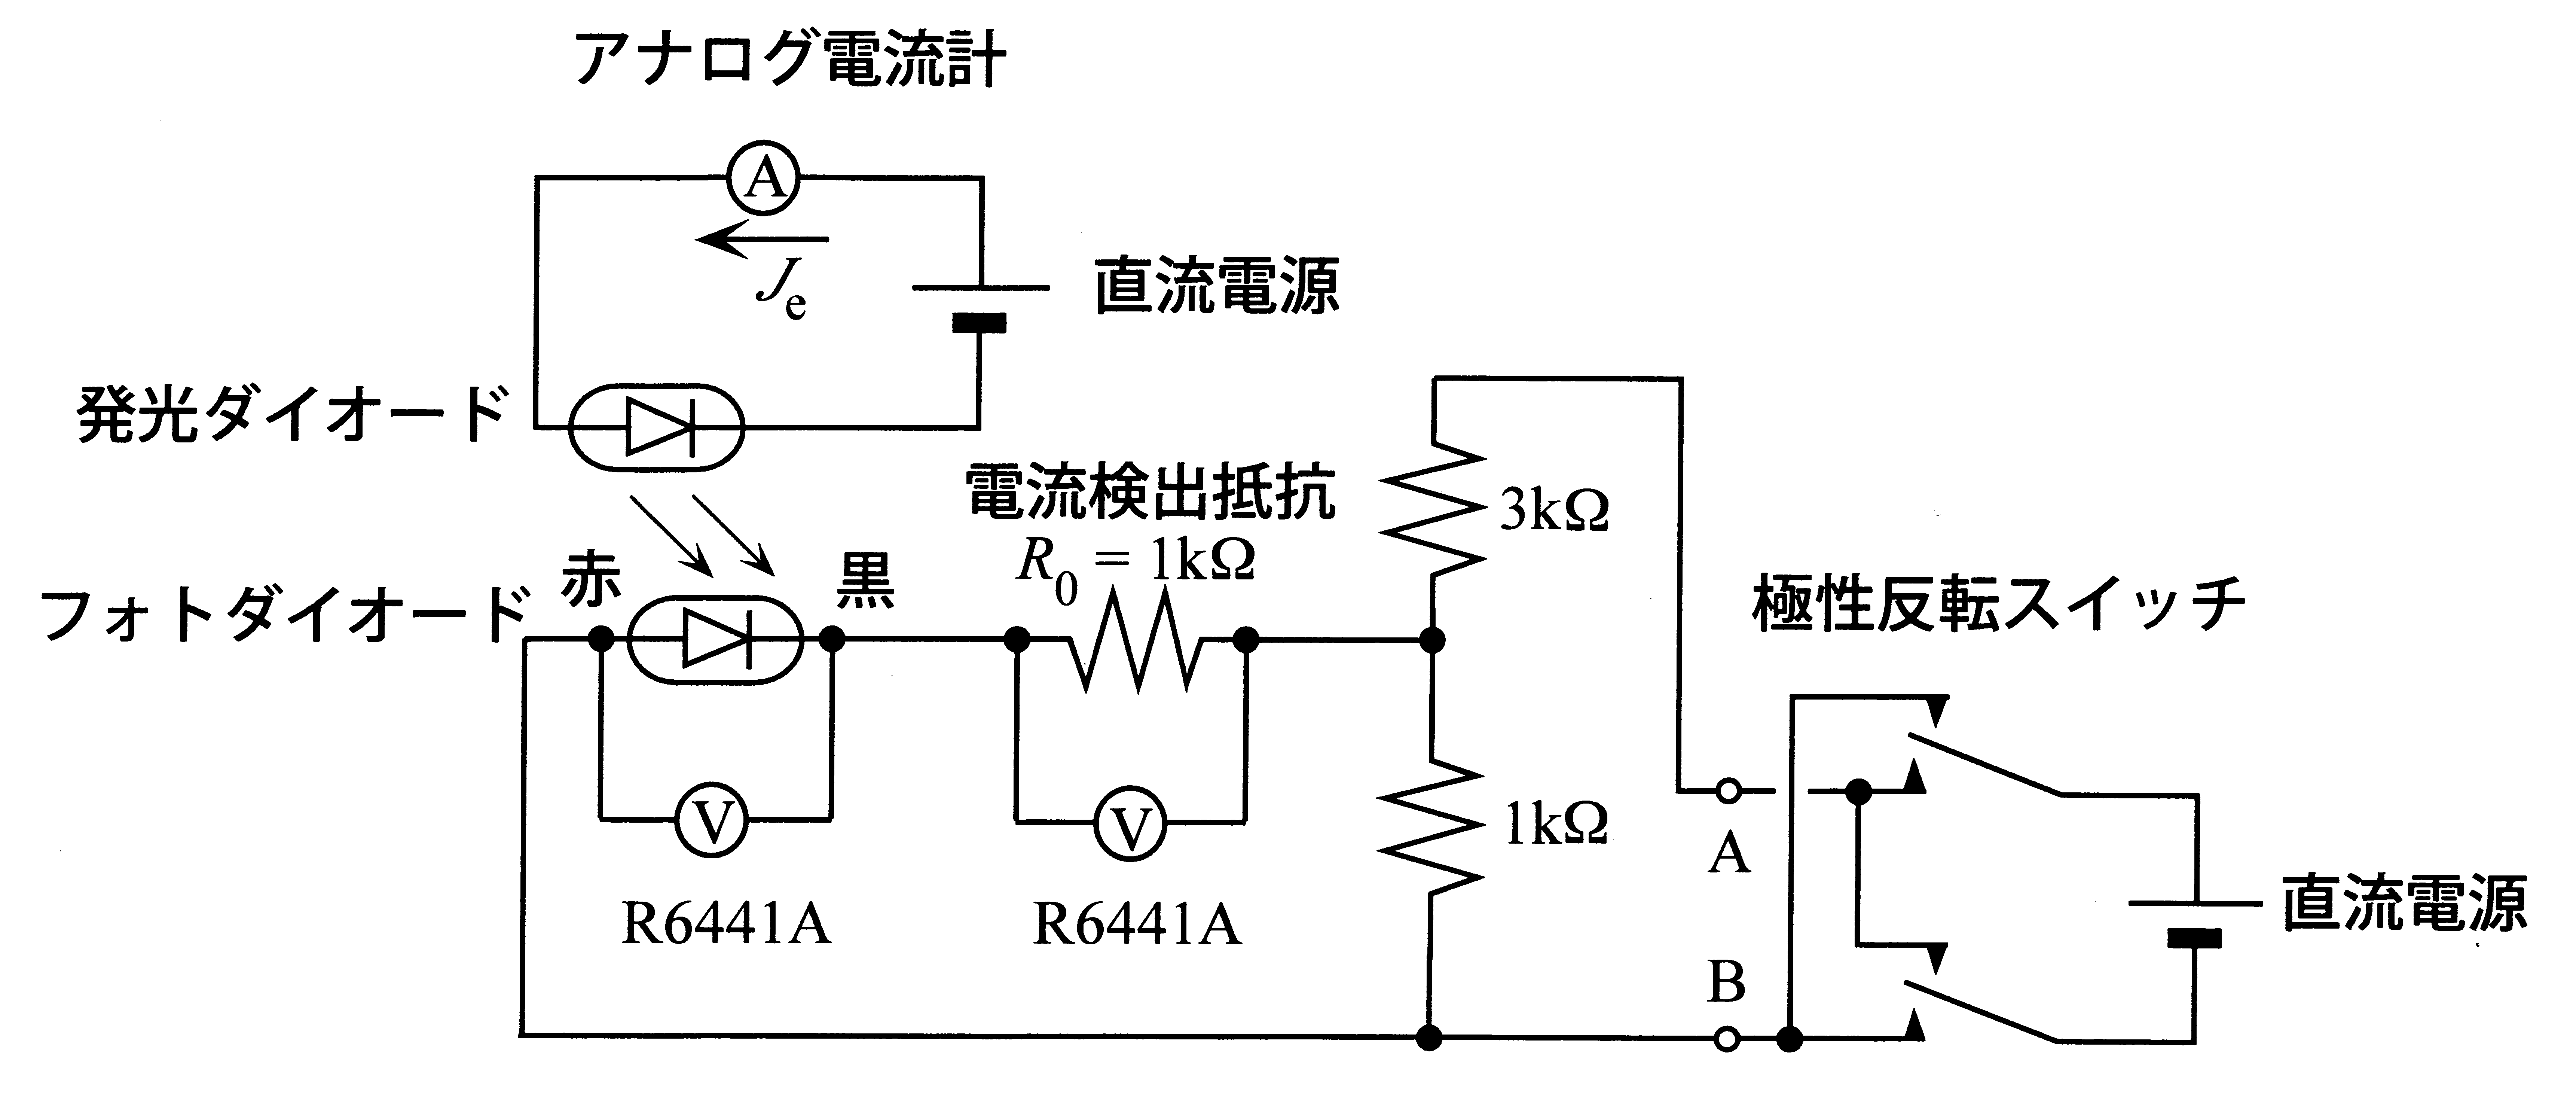
\includegraphics[width=0.8\hsize]{./photodiode_setup.eps}
    \caption{フォトダイオードの電圧電流特性測定回路}
     \label{fig:photodiode_setup}
   \end{center}
\end{figure}

\subsubsection{太陽電池の電圧電流特性}
フォトダイオードの電圧電流特性の測定実験と同様である。図\ref{fig:solor_cell_setup}に太陽電池の電圧電流特性実験のの回路図を示す。太陽電池に入射する光の光源には白熱電球を用いて、その電球光源の電源を切ったときと、点けた時の太陽電池の電圧電流特性を測定した。
\begin{figure}[!htbp]
   \begin{center}
    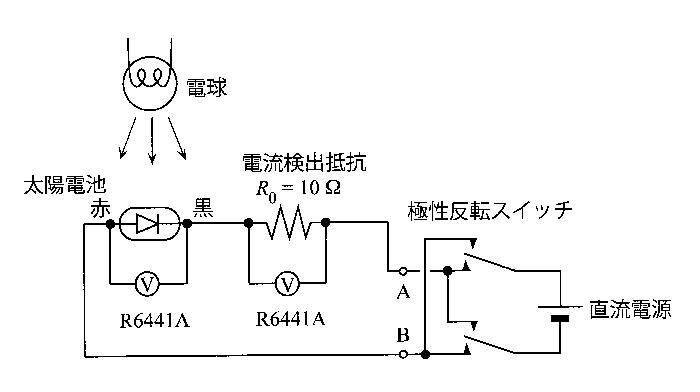
\includegraphics[width=0.7\hsize]{./solor_cell_setup.eps}
    \caption{太陽電池の電圧電流特性回路}
     \label{fig:solor_cell_setup}
   \end{center}
\end{figure}

\subsection{導電率とHall係数の測定}
電荷$q$を持つキャリアが密度$n$で半導体中に存在するとする。
キャリアの運動を説明するために、Drudeのモデルを仮定する。すなわち平均速度$v$で移動するキャリア(有効質量$m$)は、統計的に見ると一定時間$\tau$ごとに散乱されるとする。このとき物質中の電場$E$と電流密度$j=nqv$は比例関係にある(オームの法則)。
\begin{equation} 
j = \sigma E
\label{eq:conductivity}
\end{equation}
ここで比例係数$\sigma$は導電率と呼ばれる。
また電磁場中でキャリアにLorentz力$F = qE + j \times B$が働く。
このとき導電率$\sigma$はキャリア濃度$n$と移動度$\mu=q\tau/m$によって次のように表される。
\begin{equation}
\sigma = n q \mu
\label{eq:sigma}
\end{equation}

定常状態で半導体内部のローレンツ力は0となる。流れる電流と磁場が直交しているとき、それらにさらに直交する方向にローレンツ力を打ち消す電場が誘起される。これをHall電場と呼ぶ。Hall電場$E_{Hall}$は磁束密度$B$と電流密度$j$に比例し、その比例係数$R_H$をHall係数と呼ぶ。ここでHall係数$R_H$はキャリア濃度によって次のように表される。
\begin{equation}
R_H = \frac{1}{nq} 
\label{eq:R_H}
\end{equation}
このHall係数の符号から、主に伝導に寄与するキャリアの電荷の符号が分かる。

導電率$\sigma$に関する表式\ref{eq:sigma}と移動度$\mu$に関する表式\ref{eq:R_H}から、導電率$\sigma$とHall係数$R_H$が求まると、キャリア濃度$n$と移動度$\mu$が求まる。


図\ref{fig:photodiode}に本実験に用いた試料の模式図を示す。電圧は1-2端子間に印加されて、磁場は紙面に対して垂直に印加される。このときの3-4端子間の電圧を計測することで導電率を計算し、5-6端子間の電圧を計測することでHall係数を計算する。
\begin{figure}[!htbp]
   \begin{center}
    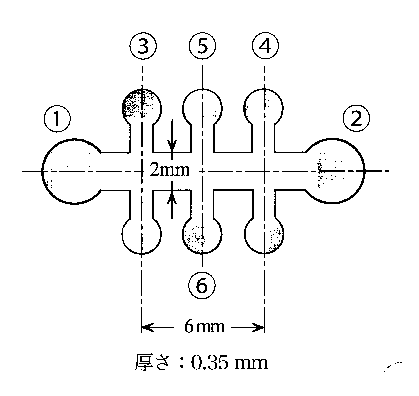
\includegraphics[width=0.4\hsize]{./sample.eps}
    \caption{資料の模式図}
     \label{fig:photodiode}
   \end{center}
\end{figure}

\subsubsection{室温での導電率とHall係数}
\label{sigma_RH_RT}
まず試料に磁場は印加せずに、室温で導電率を測定した。直流電圧を1-2端子間(図\ref{fig:photodiode})に印加し、1-2端子間に流れる電流と3-4端子間の電圧を計測した。印加電圧(1-2端子間)と流れる電流(3-4端子間)の間には線形な関係があると仮定して、回帰分析を行うことで導電率を推定した。
次に試料に磁場63mTを印加したときの、室温での導電率を同様に測定した。

室温でのHall係数は以下の手続きにより計測した。まず磁場を試料表面に垂直に印加する。このとき試料と磁場との方向関係はHall起電圧が最大となるように調整した。直流電流を1-2端子間(図\ref{fig:photodiode})に流し、5-6端子間に誘起される電圧$V_+$を計測した。次に磁場の向きを反転させて5-6端子間に誘起される電圧$V_-$を同様に測定した。我々の実験では、例えば5-6端子間が電流の流れる方向に対して傾いて接着され、抵抗によう電圧降下の影響が5-6端子間電圧に現れるなどの問題が避けられない。そこで、そのような効果をキャンセルするために我々は$(V_+-V_-)/2$をHall電圧として採用した。
Hall電場$E_{Hall}$と流れた電流密度$j$、印加した磁場$B$の関係からHall係数が計算できる。磁場の大きさを代えた場合についても測定を行い、その場合もHall係数を計算した。

\subsubsection{導電率、キャリア濃度、移動度の温度依存性}
液体窒素と熱交換できるようにした試料をヒーターで温めることで、試料の温度調節を行った。

我々の実験条件で導電率は印加する磁場の大きさに大きく依存しないと仮定してよい(この仮定は\ref{sigma_RT}章で正当付けられる)。我々は磁場を印加せずに導電率の測定を行った。温度を変化させながら図\ref{fig:photodiode}の1-2端子間に流れる電流と3-4端子間の電圧を計測し、導電率を計算した。温度を固定した際、この手続きは室温での導電率の測定実験(\ref{sigma_RH_RT}s章)と同様である。

Hall係数の温度依存性の測定の手続きについても、温度を変化させて値をひとつ取り固定したあとは、室温におけるHall係数の測定実験(\ref{sigma_RH_RT}章)と同様である。それぞれの温度でHall電場$E_{Hall}$と流れた電流密度$j$、印加した磁場$B$の関係からHall係数を計算した。

\section{実験結果}
\subsection{ダイオード}
\subsubsection{発光ダイオードの発光特性}
発光ダイオードに電圧を印加したとき、発光を肉眼で確認できる最小の電圧を、青色と緑色、赤色の発光ダイオードについてそれぞれ測定した。表\ref{tab:photodiode}に示した電圧以下で発光は確認できなかった。赤色の発光ダイオードとその他の色の発光ダイオードを比べると、発光が確認できた最小の印加電圧は赤色が小さい。また発光ダイオードに印加する電圧を大きくしたとき、発光ダイオードに流れる電流は大きくなり、同時に明るく発光した。

\begin{table}[!htbp]
   \begin{center}
  \begin{tabular}{ccc}
    青 & 緑 & 赤\\ \hline
    2.6 V & 2.7 V & 1.5 V\\
  \end{tabular}
  \label{tab:photodiode}
     \end{center}
       \caption{発光ダイオードの発光が確認できた最小の印加電圧}
\end{table}

\subsubsection{フォトダイオードの電圧電流特性}
図\ref{fig:photodiode}にフォトダイオードの電圧電流特性をプロットした。
逆方向電圧を0Vから1Vまでの範囲でフォトダイオードに印加すると、$J_e$のそれぞれについて流れる逆方向電流は飽和しほぼ一定値をとった。

表\ref{tab:Je_Vo_Js}に開放電圧値$V_0$($J=0$となる電圧値)と短絡電流値$J_s$($V=0$となる電流値)を示し、図\ref{fig:Je_Js}と図\ref{fig:Je_V0}にプロットした。
発光ダイオードに流れる電流$J_e$が大きくなるほど、開放電圧$V_0$が大きくなり、短絡電流$J_s$が小さくなった。

\begin{figure}[!htbp]
   \begin{center}
    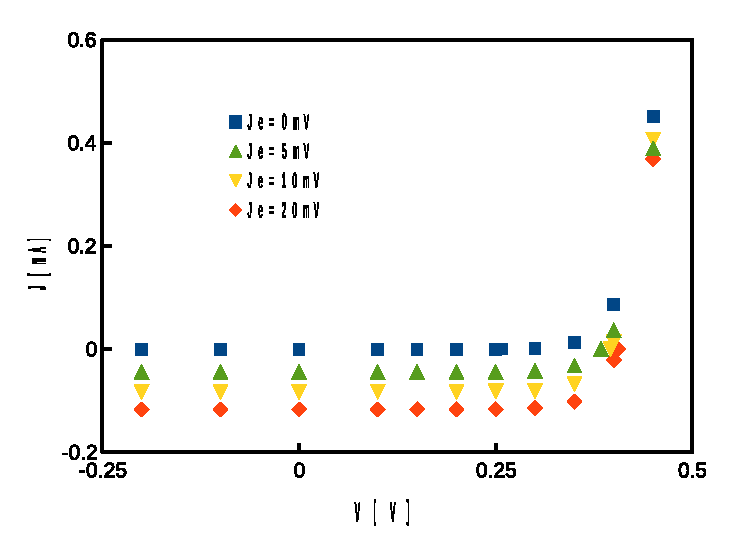
\includegraphics[width=0.8\hsize]{./photodiode.eps}
    \caption{フォトダイオードの電圧電流特性}
     \label{fig:photodiode}
   \end{center}
\end{figure}
\begin{table}[!htbp]
   \begin{center}
  \begin{tabular}{ccc}
    $J_e$ [mA]  & $V_0$ [V] & $J_s$ [mA]\\ \hline
    0 & 0.267 & -0.0004 \\
    5 & 0.384 & -0.0445 \\
    10 & 0.396 & -0.0832 \\
    20 & 0.405 & -0.0117 \\
  \label{tab:Je_Vo_Js}
  \end{tabular}
     \end{center}
       \caption{$J_e$に対する開放電圧$V_0$と短絡電流$J_s$}
\end{table}
\begin{figure}[htbp]
 \begin{minipage}{0.5\hsize}
  \begin{center}
   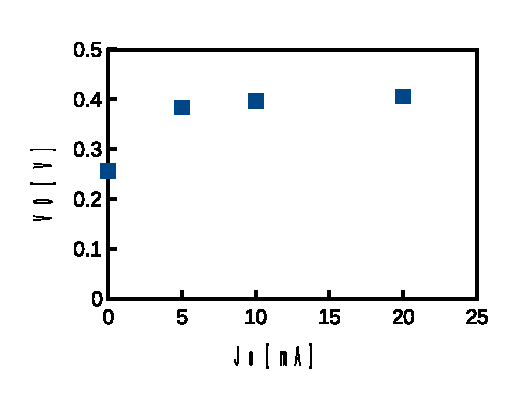
\includegraphics[width=80mm]{Je_V0.eps}
  \end{center}
  \caption{$J_e$と開放電圧$V_0$の関係}
  \label{fig:Je_V0}
 \end{minipage}
 \begin{minipage}{0.5\hsize}
  \begin{center}
   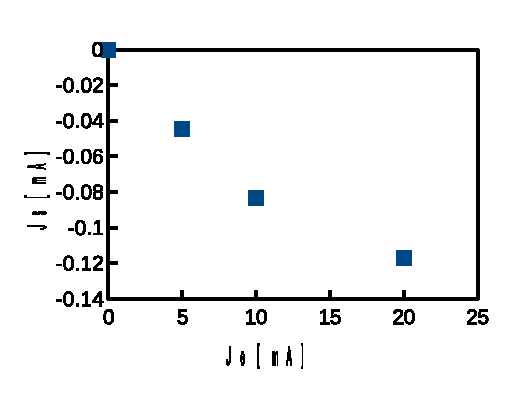
\includegraphics[width=80mm]{Je_Js.eps}
  \end{center}
  \caption{$J_e$と短絡電流$J_s$の関係}
  \label{fig:Je_Js}
 \end{minipage}
\end{figure}

\subsubsection{太陽電池の電圧電流特性}
図\ref{fig:solor_cell}に太陽電池の電圧電流特性をプロットした。開放電圧$V_0$は0.50V、短絡電流$J_s$は-52.1mAだった。表\ref{tab:Je_Vo_Js}に示したフォトダイオードの電圧電流特性と比較すると、太陽電池は光を照射した際に大きな開放電圧$V_0$と大きな短絡電流$J_s$の絶対値をもつ。
 \begin{figure}[!htbp]
   \begin{center}
    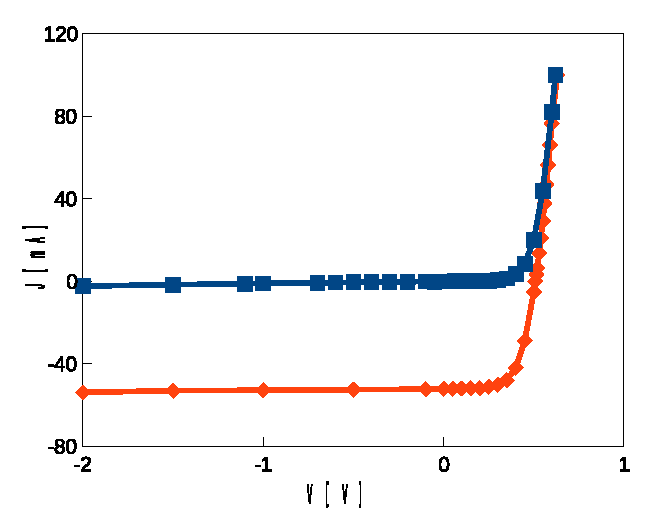
\includegraphics[width=0.6\hsize]{./solor_cell.eps}
    \caption{}
     \label{fig:solor_cell}
   \end{center}
\end{figure}

\subsection{導電率とHall係数の測定}

\subsubsection{室温での導電率とHall係数}
室温での半導体試料の電圧電流特性を図\ref{fig:conductivity_RT}にプロットした。このとき試料に磁場は印加していない。印加した電圧が0Vから0.25Vの間では流れる電流との間に線形性が保たれていることが分かる。
導電率$\sigma$は線形関数の傾きの逆数に比例しその値を$25.69\pm0.10$ [mS/m]と見積もった。試料に63mTの磁場を印加した場合も同様に電気導電率を計算すると、その値は$25.93\pm0.06$ [mS/m]だった。十分に強い磁場を印加すると、電気伝導度はその測定誤差よりも大きな値シフトすることが分かる。

Hall係数の測定結果を表\ref{tab:Hall}に示す。Hall係数は室温で$-1.10\pm0.04\times10^{-3}[m^3/C]$だった。

計測した導電率とHall係数から室温での移動度は0.35[$m^2V^{-1}s^{-1}$]程度と見積もった。

\begin{figure}[!htbp]
   \begin{center}
    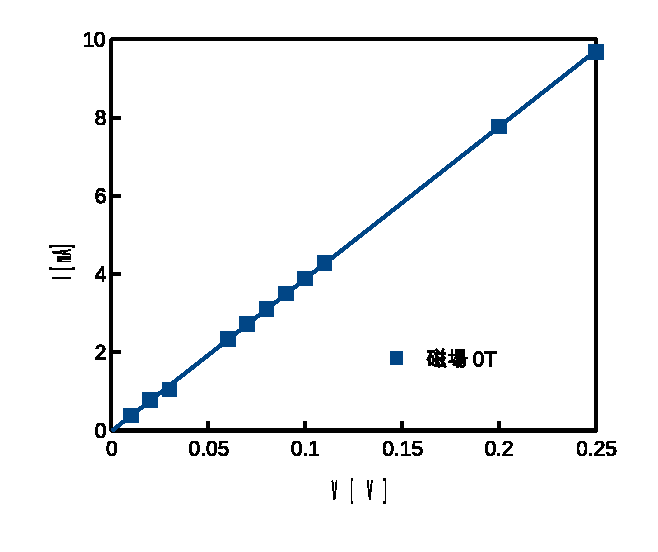
\includegraphics[width=0.5\hsize]{./conductivity_RT.eps}
    \caption{試料の室温での電圧電流特性}
     \label{fig:conductivity_RT}
   \end{center}
\end{figure}

\begin{table}[!htbp]
   \begin{center}
  \begin{tabular}{ccc}
    $B [mT]$  & $j [A/m^2]$ & $R_H [m^3/C]$\\ \hline
    63 & 714 & -0.00106 \\
    102 & 143 & -0.00108 \\
    51 &143 & -0.00116 \\
  \end{tabular}
  \label{tab:Hall}
     \end{center}
       \caption{室温でのHall係数の測定値}
\end{table}

\subsubsection{導電率、キャリア密度、移動度の温度依存性}
図\ref{fig:T_sigma}と図\ref{fig:T_R}に、測定した導電率とホール係数の温度特性をそれぞれプロットした。温度が大きくなるにつれて、Hall係数と導電率は小さくなった。
\begin{figure}[htbp]
 \begin{minipage}{0.5\hsize}
   \begin{center}
    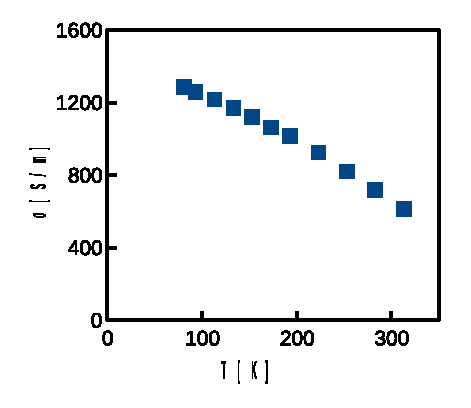
\includegraphics[width=0.8\hsize]{./T_sigma.eps}
    \caption{導電率の温度特性}
     \label{fig:T_sigma}
   \end{center}
 \end{minipage}
 \begin{minipage}{0.5\hsize}
   \begin{center}
    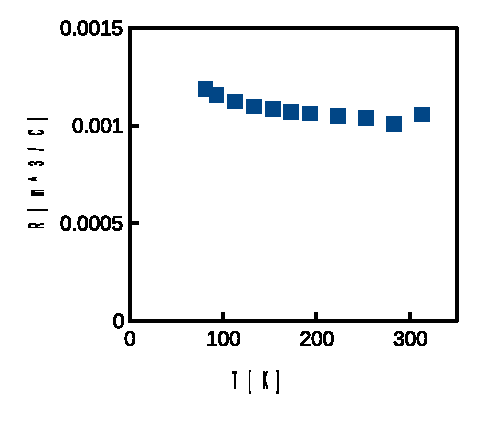
\includegraphics[width=0.8\hsize]{./T_R.eps}
    \caption{ホール係数の温度特性}
     \label{fig:T_R}
   \end{center}
 \end{minipage}
\end{figure}


図\ref{fig:T_n}と図\ref{fig:T_mu}にキャリア密度$n$と移動度$\mu$をそれぞれプロットした。温度を大きくしてゆくと、キャリア密度は大きくなり移動度は小さくなることがわかる。
特に移動度の温度依存を定量的にさらに分析するために、図\ref{fig:T_mu_log}に移動度を両対数プロットした。
70Kから200K程度の温度で、おおむね$\mu \sim T^{1/2}$が見てとれる。また200K以上の温度で、おおむね$\mu \sim T^{3/2}$が見てとれる。
\begin{figure}[htbp]
 \begin{minipage}{0.5\hsize}
   \begin{center}
    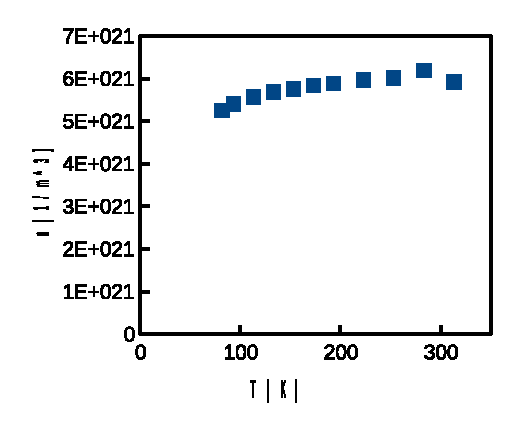
\includegraphics[width=0.8\hsize]{./T_n.eps}
    \caption{キャリア密度の温度特性}
     \label{fig:T_n}
   \end{center}
 \end{minipage}
 \begin{minipage}{0.5\hsize}
   \begin{center}
    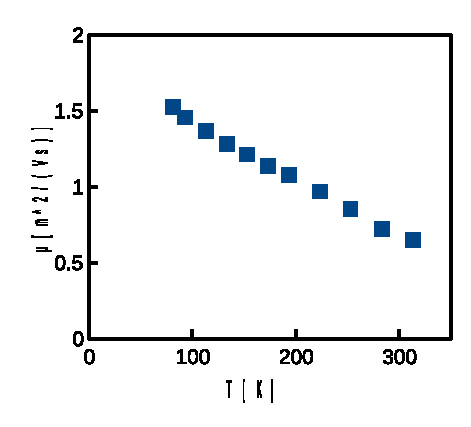
\includegraphics[width=0.8\hsize]{./T_mu.eps}
    \caption{移動度の温度特性}
     \label{fig:T_mu}
   \end{center}
 \end{minipage}
\end{figure}

 \begin{figure}[!htbp]
   \begin{center}
    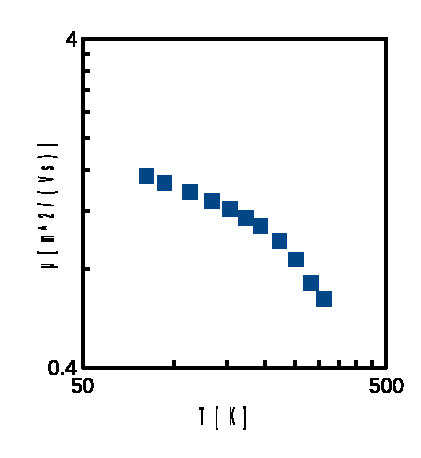
\includegraphics[width=0.4\hsize]{./T_mu_log.eps}
    \caption{移動度の温度特性(両対数プロット)}
     \label{fig:T_mu_log}
   \end{center}
\end{figure}

\section{考察}
\subsection{ダイオード}
\subsubsection{発光ダイオードの発光特性}
発光ダイオードの発光が確認できた最小の印加電圧は、青色で2.6V、緑色で2.7V、赤色で1.5Vだった。この電圧を波長に換算すると、青色のダイオードで477nm、緑色で460nm、赤色で827nmである。これは実際に変換された光の波長と同程度である。したがって、発光ダイオードの動作原理がバンド間遷移(準位間遷移)によるものであると確かめられた。

\subsubsection{フォトダイオードの電圧電流特性}
発光ダイオードに流れる電流$J_e$が大きくなればなるほど、フォトダイオードの開放電圧$V_0$は大きくなるが、$V_0$は増加とともに飽和してゆく。開放電圧$V_0$はn型半導体中の電子とp型半導体中の電子の化学ポテンシャルの差に対応するため、この電圧の飽和は化学ポテンシャルの飽和を意味する。

また電流$J_e$が大きくなればなるほど、フォトダイオードの短絡電流$V_0$も大きくなった。この短絡電流は光電流と再結合電流が釣り合って平衡状態に達したとき流れる電流である。

\subsubsection{太陽電池の電圧電流特性}
フォトダイオードの電圧電流特性と太陽電池の電圧電流特性を比較すると、太陽電池は大きな開放電圧$V_0$と絶対値が大きな短絡電流$J_s$を持つ。この二つの積$V_0J_s$は太陽電池の発電力を意味するため\footnote{正確には図\ref{fig:solor_cell}のように電圧電流特性をプロットしたとき、グラフ上の第3象限の点における$-VJ$が発電力である。この$-VJ$の最大値はおおむね$V_0$と$J_s$の値で決まる。}、太陽電池が(フォトダイオードに比べて)効率よく発電できることを意味する。

\subsection{導電率とHall係数の測定}
\subsubsection{室温での導電率とHall係数}\label{sigma_RT}
\label{sigma_RT}
試料に磁場を印加しなかったときと、63mTの磁場を印加したときで、室温の導電率はそれぞれ$25.69\pm0.10$ [mS/m]と$25.93\pm0.06$ [mS/m]と見積もった。この二つの測定値の差は偶然誤差の範囲では説明できず、有意であると筆者は考える。しかし我々がHall係数の測定実験で扱う磁場の強さを考えたとき、導電率がかけた磁場に依存して変化する影響は無視できる。したがって我々は磁場を印加しない条件で導電率の温度依存性を測定した。

室温計測されたHall係数は$-1.10\pm0.04\times10^{-3}[m^3/C]$だった。Hall抵抗の符号が負をとったことから試料はn型半導体である。また導電率とHall係数から計算した移動度は0.35程度と見積もった。
この値はGeの伝導電子の移動度0.36と近い値を持つため、本実験で用いた試料はGeを用いたものと推定した。

\subsubsection{導電率、キャリア濃度、移動度の温度依存性}
図\ref{fig:T_n}から温度が上がるとキャリア密度$n$も上がることが分かる。これは以下の理論式でモデル化される。
\begin{equation}
n = 2 (2 \pi m k_B T / h^2)^{3/2} exp(-\frac{E_G}{2k_BT}-\frac{E-E_f}{k_BT})
\label{eq:C1-18}
\end{equation}
ここで$E_G$はバンドギャップ、$E_f$はフェルミ準位である。

図\ref{fig:T_mu}、\ref{fig:T_mu_log}から温度が上がると、移動度は小さくなることが分かる。この移動度は70Kから200K程度の温度でおおむね$\mu \sim T^{-1/2}$であり、また200K以上の温度でおおむね$\mu \sim T^{-3/2}$といえる。
200K以上の温度でおおむね移動度$\mu$がTの$-3/2$乗に比例することは、電子の格子振動による散乱(フォノン散乱)の効果が支配的であるとして説明できる。

\section{結論}
発光ダイオードやフォトダイオード、太陽電池の光デバイスの動作を実験で調べた。発光ダイオードの動作がバンド間遷移であることが確認できた。また電子の化学ポテンシャル(フェルミ準位)を用いてフォトダイオードの動作が説明できることが分かった。太陽電池の発電力が最大となる条件を求めた。また半導体試料のキャリア密度と移動度の温度依存性を磁場下で実験した。室温での移動度の測定から試料がGeであると推定した。移動度は温度200K以上で温度の-3/2乗に比例することが分かった。



\end{document}